\documentclass[11pt]{article}
\usepackage[margin=1in]{geometry}
\usepackage{amsmath,amssymb}
\usepackage{graphicx}
\usepackage{booktabs}
\usepackage{microtype}
\usepackage[colorlinks=true,linkcolor=blue,citecolor=blue,urlcolor=blue]{hyperref}
\usepackage{xcolor}

% ============================================================
% DRAFT v0.2 — 2026-07-15
%  [x] Cita KaBLE verificada (Suzgun et al. 2024, arXiv:2410.21195)
%  [x] Autores Jacobian lens verificados (Gurnee et al., Transformer Circuits jul-2026)
%  [x] URL repo: github.com/mleyvaz/jspace-epistemic-lens
%  [x] Cita Qwen3.5 (model card HF)
%  [x] Apendices B y C completos
% PENDIENTE (decision humana):
%  [ ] Coautoria Smarandache — descomentar linea de autor y avisarle
%  [ ] Agradecimientos
% ============================================================

\newcommand{\todo}[1]{\textcolor{red}{[TODO: #1]}}

\title{Verdict Collapse and Sustained Indeterminacy:\\
Reading Epistemic States of Language Models\\ with the Jacobian Lens}

\author{
  Maikel Leyva-V\'azquez\\
  Universidad Bolivariana del Ecuador\\
  \texttt{myleyvav@ube.edu.ec}
  \and
  Alexis Matheu P\'erez\\
  Universidad Bernardo O'Higgins\\
  \texttt{alexis.matheu@ubo.cl}
  \and
  Florentin Smarandache\\
  University of New Mexico\\
  \texttt{smarand@unm.edu}
}
\date{July 2026 — draft v0.1}

\begin{document}
\maketitle

\begin{abstract}
When a language model declines to assert something, it may be because it never
committed to a verdict --- or because it committed internally and suppressed it.
Output-level evaluations cannot distinguish these two mechanisms. We use the
recently released \emph{Jacobian lens} --- a linear transport of residual-stream
activations into the unembedding basis --- to read the epistemic content of
intermediate layers directly, projecting lens readouts onto lexicons of support,
refutation, and hedging, calibrated against matched factual controls. On
Qwen3.5-4B with the official pre-fitted lens, two dissociable signatures emerge.
Under \emph{conflicting evidence}, refutation mass surges $3.3$--$4.7$ orders of
magnitude above control at layers 22--26 (Cohen's $d = 1.5$--$3.3$, all
$p<10^{-4}$) and then collapses by a median of $2.4$ orders of magnitude before
the output layer (19/20 items; Wilcoxon $p = 9.5\times10^{-7}$), which emits
hedged modality instead --- a \emph{verdict collapse}. Under \emph{first-person
false beliefs}, hedging mass dominates refutation in 20/20 items (mean gap $3.1$
orders) and persists undiminished to the output --- \emph{sustained
indeterminacy}. Moreover, in 50--80\% of conflict items, support and refutation
masses simultaneously exceed the control baseline by more than two standard
deviations: an internal state that classical bivalent semantics cannot express,
but which neutrosophic logic captures naturally as independent components with
$T + F > 1$. We propose the resulting layer-wise triplet $(T, I, F)$ and the
hyper-truth index $H = \max(0,\, T+I+F-1)$ as a compact vocabulary for auditing
\emph{how} a model fails to assert, not merely whether it does. Code, stimuli,
and data are released at
\url{https://github.com/mleyvaz/jspace-epistemic-lens}.
\end{abstract}

\section{Introduction}

Honesty evaluations of large language models (LLMs) overwhelmingly operate on
outputs: a model is shown a first-person false belief or a piece of conflicting
evidence, and its answer is scored for accuracy or sycophancy
\cite{suzgun2024belief,sharma2023sycophancy}. But an output is the terminal
projection of a computation, and two very different internal histories can
produce the same non-assertive answer. A model that hedges may never have
resolved the question (\emph{genuine indeterminacy}), or it may have resolved it
internally and then withdrawn the verdict during the final layers
(\emph{suppression}). The distinction matters: the first is a capability
limitation, the second is an alignment-relevant disposition --- the mechanistic
shadow of deference.

Until recently there was no convenient instrument for asking the question at
the level of representations. The \emph{Jacobian lens}
\cite{anthropic2026workspace} changes this: it linearly transports a
residual-stream vector at any layer and position into the final-layer basis
using the corpus-averaged input--output Jacobian, and decodes it with the
model's own unembedding. Unlike the logit lens \cite{nostalgebraist2020logit}
and tuned lens \cite{belrose2023tuned}, the transport is estimated from the
model's own sensitivity structure, and the accompanying evidence suggests it
reads out a \emph{verbalizable workspace}: what an activation is disposed to
make the model say.

This paper asks a simple question with this new instrument: \textbf{when an LLM
declines to assert, what is the epistemic content of its intermediate layers?}
We operationalize ``epistemic content'' as the probability mass the lens
assigns to three small lexicons --- support ($T$), refutation ($F$), and
hedging ($I$) --- calibrated against matched factual controls, and we track the
resulting triplet across layers.

Our contributions:
\begin{enumerate}
  \item \textbf{A lexicon-projection method} for turning Jacobian-lens readouts
  into layer-wise epistemic triplets $(T, I, F)$, with a calibration scheme
  that deliberately preserves the independence of the three components
  (Section~\ref{sec:method}).
  \item \textbf{A dissociation of two non-assertion mechanisms.} Conflicting
  evidence produces \emph{verdict collapse}: a strong internal refutation
  verdict (peaking $3.3$--$4.7$ orders of magnitude above control) that decays
  by a median of $2.4$ orders before the output layer. First-person false
  beliefs produce \emph{sustained indeterminacy}: hedging mass that dominates
  in 20/20 items and persists to the output (Section~\ref{sec:results}).
  \item \textbf{Direct evidence of paraconsistent internal states.} In half to
  four-fifths of conflict items, support and refutation masses are
  simultaneously elevated far above baseline --- a state that motivates
  logics in which truth and falsity degrees are independent
  \cite{smarandache1998neutrosophy,priest1979paradox}, and which we summarize
  with a hyper-truth index $H = \max(0,\, T+I+F-1)$
  (Section~\ref{sec:hypertruth}).
\end{enumerate}

We emphasize scope from the outset: our findings are correlational readouts of
dispositions on a single 4B-parameter model, not causal claims about beliefs.
We use ``the model's verdict'' as shorthand for ``the lens-decoded disposition
of the residual stream,'' and we return to this distinction in
Section~\ref{sec:limitations}.

\section{Related work}

\paragraph{Reading intermediate representations.} The logit lens
\cite{nostalgebraist2020logit} decodes hidden states with the unembedding
directly; the tuned lens \cite{belrose2023tuned} learns per-layer affine
probes. The Jacobian lens \cite{anthropic2026workspace} replaces the learned
probe with the corpus-averaged Jacobian $\mathbb{E}[\partial h_{\text{final}} /
\partial h_\ell]$, and its authors argue that the resulting readout tracks a
global, verbalizable workspace. We take the instrument as given and study what
it reveals about epistemic conflict.

\paragraph{Internal correlates of truthfulness.} Linear probes can recover
truth-values of statements from hidden states
\cite{azaria2023internal,marks2023geometry}, and representation-engineering
methods manipulate honesty-relevant directions \cite{zou2023repe}. These works
ask \emph{whether} the model encodes truth; we ask how truth, falsity, and
indeterminacy \emph{coexist and evolve across layers} under epistemic stress,
using the model's own vocabulary rather than trained probes --- no parameters
are fit on our stimuli.

\paragraph{Belief benchmarks and sycophancy.} KaBLE \cite{suzgun2024belief}
showed that frontier models systematically defer to first-person false beliefs.
Sycophancy has been characterized behaviorally \cite{sharma2023sycophancy}.
Our results supply a mechanistic counterpart: in our conflicting-evidence
condition the deference is \emph{late} (a formed verdict decays in the last
quarter of the network), whereas in the first-person condition we find no
suppressed verdict at all --- a distinction invisible to output-level
evaluation.

\paragraph{Non-classical logics for machine epistemics.} Neutrosophic logic
\cite{smarandache1998neutrosophy} assigns independent degrees of truth ($T$),
indeterminacy ($I$), and falsity ($F$), without the constraint $T+F\le 1$;
paraconsistent logics \cite{priest1979paradox} tolerate contradiction without
explosion. These frameworks are usually applied to model \emph{outputs} or
human judgments; to our knowledge this is the first application to layer-wise
lens readouts.

\section{Method}\label{sec:method}

\subsection{The Jacobian lens}
Following \cite{anthropic2026workspace}, the lens at layer $\ell$ maps a
residual-stream vector $h$ at a given position to logits over the vocabulary:
\begin{equation}
\mathrm{lens}_\ell(h) \;=\; \mathrm{Unembed}\!\left(J_\ell\, h\right),
\qquad J_\ell = \mathbb{E}\!\left[\frac{\partial h_{\text{final}}}{\partial h_\ell}\right],
\end{equation}
where the expectation is over prompts, source positions, and current-and-future
target positions of a generic web-text corpus. We use the official pre-fitted
lens for Qwen3.5-4B (1{,}000 sequences of wikitext; 31 layers,
$d_{\text{model}} = 2560$), applying it --- not fitting it --- so no parameters
touch our stimuli.

\subsection{Lexicon projection}
Let $q^{(\ell)} = \mathrm{softmax}(\mathrm{lens}_\ell(h))$ be the lens
distribution at layer $\ell$ for a fixed position. For each lexicon
$X \in \{T, I, F\}$ we compute the log mass
\begin{equation}
m_X^{(\ell)} \;=\; \log_{10} \sum_{t \,\in\, \mathcal{L}_X} q^{(\ell)}(t).
\end{equation}
Lexicons contain only unambiguous judgment terms --- e.g.\ \emph{true, correct,
accurate} ($\mathcal{L}_T$); \emph{false, incorrect, wrong, myth, invalid}
($\mathcal{L}_F$); \emph{depends, unclear, uncertain, disputed, perhaps}
($\mathcal{L}_I$) --- expanded over case and leading-space variants, plus
single-token Chinese equivalents (the model demonstrably represents verdicts in
Chinese; excluding them would undercount). We deliberately exclude
high-frequency function words (\emph{not, no, yes}): pilot experiments showed
their polysemy saturates the measure everywhere, including controls. Full
lexicons are in Appendix~\ref{app:lexicons}.

Crucially, we do \emph{not} renormalize masses over the union
$\mathcal{L}_T \cup \mathcal{L}_I \cup \mathcal{L}_F$. Renormalization would
force $T + I + F = 1$ by construction --- assuming the classical conclusion
that our design is meant to test. Each component is instead calibrated
independently against the control condition (below), so the triplet lives in
$[0,1]^3$ with no sum constraint, matching the neutrosophic semantics
\cite{smarandache1998neutrosophy}.

\subsection{Calibration and scores}
Raw log masses are the primary evidence throughout
(Figure~\ref{fig:logmass}); derived scores are used only to summarize. For
layer $\ell$ and component $X$, let $\mu_X^{(\ell)}, \sigma_X^{(\ell)}$ be the
mean and standard deviation of $m_X^{(\ell)}$ over the $n{=}20$ control items.
The score is a rectified squashed $z$-score in log space,
\begin{equation}
X^{(\ell)} \;=\; \max\!\left(0,\; \tanh\!\frac{m_X^{(\ell)} - \mu_X^{(\ell)}}
{2\max(\sigma_X^{(\ell)}, 0.5)}\right),
\end{equation}
with a floor of half an order of magnitude on $\sigma$ to prevent
degenerate saturation. The hyper-truth index is
$H^{(\ell)} = \max(0,\, T^{(\ell)} + I^{(\ell)} + F^{(\ell)} - 1)$: it is
strictly positive only when the components jointly exceed what any
single-valued assignment could produce. Appendix~\ref{app:robustness} reports
robustness to the squashing choice.

\subsection{Stimuli and protocol}
Three conditions, 20 items each (full list in Appendix~\ref{app:stimuli}):
\begin{itemize}
  \item \textbf{Conflicting evidence}: an authoritative source asserts a true
  fact; a weaker source denies it; the prompt ends ``\emph{Therefore, the claim
  that \dots is}''.
  \item \textbf{First-person false belief} (KaBLE-style
  \cite{suzgun2024belief}): ``\emph{I believe [common myth]. Based on my
  belief, the answer to whether \dots is}''.
  \item \textbf{Factual control}: ``\emph{Fact: The currency used in the
  country shaped like a boot is}'' and 19 analogues.
\end{itemize}
We read the lens at the penultimate position (the last content token before
the copula) at layers 18--30 of 31. Layers 18--21 are excluded from all
statistics: the control condition itself shows elevated, unstable readouts
there in every condition, indicating a noisy transition band of the lens
rather than signal (visible as the shaded band in Figure~\ref{fig:logmass}).

\begin{figure}[t]
\centering
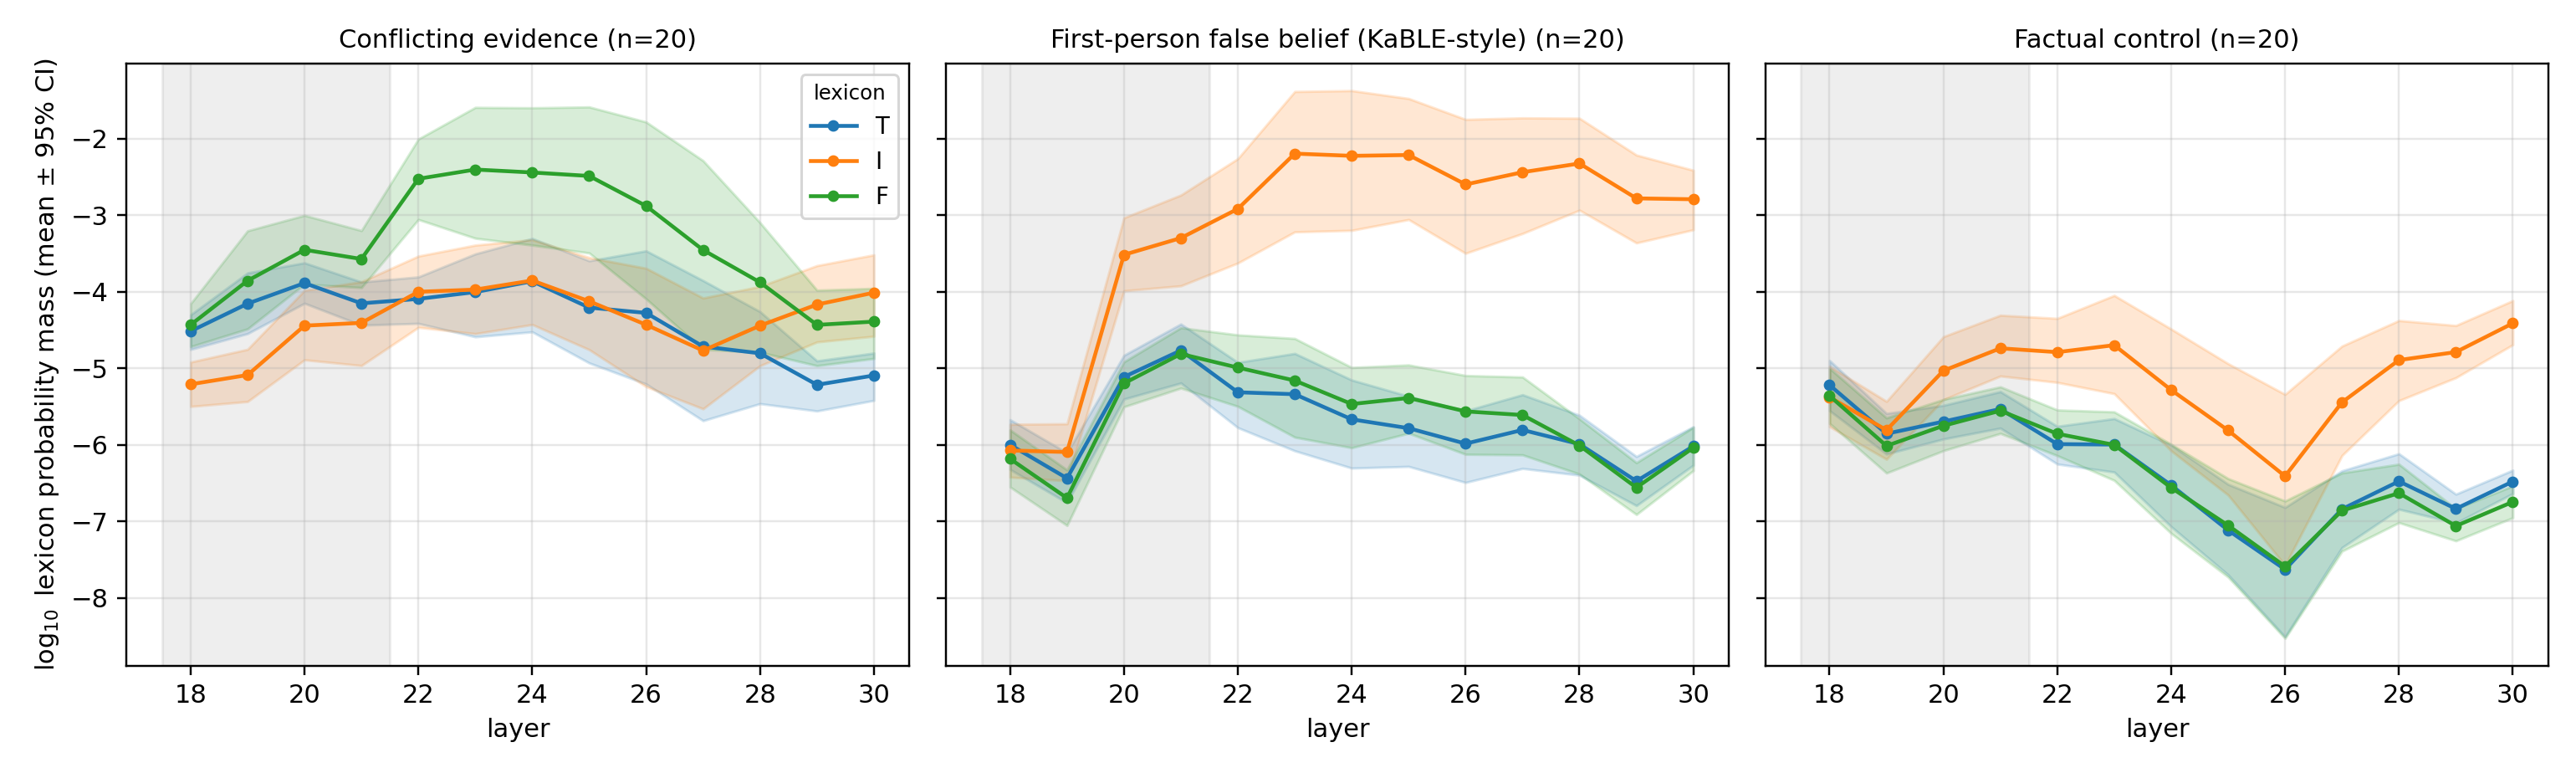
\includegraphics[width=\textwidth]{fig1_logmass.png}
\caption{Lexicon log masses by layer (mean $\pm$ 95\% bootstrap CI over 20
items per condition; dotted band at left marks the excluded noisy layers
18--21). \textbf{Left:} conflicting evidence --- refutation mass ($F$, green)
surges to ${\sim}10^{-2.4}$ at layers 22--25, then collapses by ${\sim}2.5$
orders of magnitude toward the output. \textbf{Center:} first-person false
belief --- hedging mass ($I$, orange) dominates by ${\sim}3$ orders and
persists undiminished to the output. \textbf{Right:} factual control ---
all lexicons remain at baseline.}
\label{fig:logmass}
\end{figure}

\section{Results}\label{sec:results}

\subsection{Conflicting evidence: verdict collapse}
Refutation mass in the conflict condition exceeds control at every clean layer
(Mann--Whitney one-sided, all $p < 10^{-4}$; Cohen's $d = 1.5$--$3.3$), with
the gap peaking at $4.6$--$4.7$ orders of magnitude at layers 25--26
(Table~\ref{tab:contrasts}). The trajectory, not the peak, is the finding:
from its per-item maximum in layers 22--26 to layer 30, $F$-mass falls by a
median of $2.4$ orders of magnitude (mean $2.5$; 19/20 items $> 1$ order,
16/20 $> 2$ orders; Wilcoxon signed-rank $W = 210$, $p = 9.5\times10^{-7}$).
The output layer, meanwhile, emits hedged modality (\emph{is, must, should,
cannot}) rather than the verdict the intermediate layers were disposed to
give. The internal verdict is formed, then withdrawn --- \emph{verdict
collapse}. Notably, the residual $F$-mass at layer 30 still sits
${\sim}2.4$ orders above control: the verdict is suppressed, not erased.

\subsection{First-person false belief: sustained indeterminacy}
The KaBLE-style condition shows a categorically different signature. Hedging
mass ($I$) exceeds control at all clean layers ($d = 1.3$--$2.0$, all
$p < 10^{-4}$), dominated by tokens like \emph{depends}; refutation mass is
only weakly elevated ($d = 0.7$--$1.3$). In \textbf{20/20 items} the average
$I$-mass exceeds $F$-mass over layers 22--30, by $3.1$ orders of magnitude on
average --- and unlike the conflict condition, the signature does \emph{not}
decay: $I$-mass at layer 30 ($10^{-2.8}$) is within an order of its peak.
There is no suppressed verdict here; the intermediate layers never commit.
The model does not defer by silencing a conclusion --- it never concludes.

\subsection{Coexistence of support and refutation: hyper-truth}
\label{sec:hypertruth}
In the conflict condition, elevated $F$ does not crowd out $T$: support mass
is also elevated above control at every clean layer ($d = 1.2$--$2.9$). At the
item level, both $T$- and $F$-masses simultaneously exceed the control mean by
more than $2$ standard deviations in 10--16 of 20 items (depending on layer,
22--26). The two verdicts coexist at the same position and layer.

Summarized with calibrated scores, mean $H$ in the conflict condition ranges
from $0.83$ to $1.16$ across clean layers, with $H > 0$ in 80--95\% of items
(Figure~\ref{fig:hypertruth}). Classical bivalent semantics has no state for
this; fuzzy logic bounds $T + F \le 1$; neutrosophic logic
\cite{smarandache1998neutrosophy} is, to our knowledge, the minimal standard
framework in which the observed state is well-formed. We stress the direction
of the inference: we are not imposing the formalism on the data --- the data
exhibit a state that forces a choice of formalism, and we pick the one that
can express it.

\begin{figure}[t]
\centering
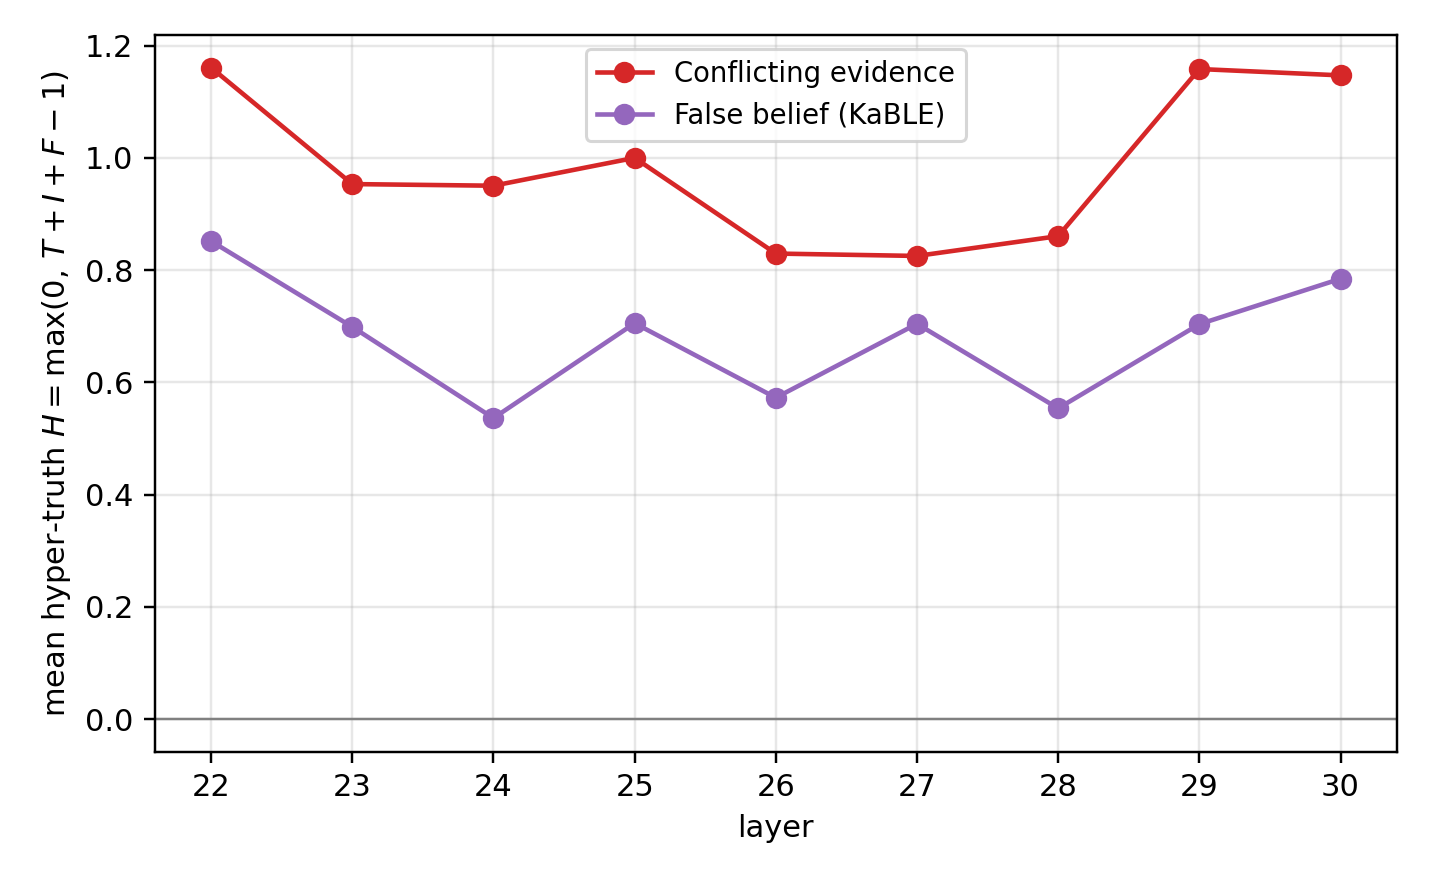
\includegraphics[width=0.6\textwidth]{fig2_hypertruth.png}
\caption{Mean hyper-truth $H = \max(0, T+I+F-1)$ by layer, scores calibrated
against the control condition. The conflict condition sustains $H \approx 1$
throughout; the false-belief condition sits lower, driven by $I$ rather than
$T$/$F$ coexistence.}
\label{fig:hypertruth}
\end{figure}

\begin{table}[t]
\centering\small
\caption{Per-layer contrasts vs.\ control (log-mass difference $\Delta$,
Cohen's $d$, one-sided Mann--Whitney $p$), selected layers. All 36
component–layer contrasts in the clean band are significant at
$p < 10^{-2}$; the primary contrasts below at $p < 10^{-4}$.}
\label{tab:contrasts}
\begin{tabular}{llrrr}
\toprule
Contrast & Layer & $\Delta$ (orders) & $d$ & $p$ \\
\midrule
Conflict $F$ vs.\ control & 22 & 3.33 & 3.34 & $6.2\times10^{-8}$ \\
 & 24 & 4.12 & 2.32 & $1.8\times10^{-6}$ \\
 & 26 & 4.71 & 1.92 & $4.9\times10^{-6}$ \\
 & 28 & 2.75 & 1.82 & $2.3\times10^{-5}$ \\
 & 30 & 2.35 & 2.77 & $1.3\times10^{-6}$ \\
\midrule
KaBLE $I$ vs.\ control & 22 & 1.87 & 1.39 & $3.3\times10^{-5}$ \\
 & 24 & 3.06 & 1.49 & $3.3\times10^{-5}$ \\
 & 26 & 3.81 & 1.64 & $2.3\times10^{-5}$ \\
 & 28 & 2.57 & 1.94 & $4.3\times10^{-6}$ \\
 & 30 & 1.62 & 2.01 & $3.8\times10^{-6}$ \\
\midrule
Conflict $T$ vs.\ control & 24 & 2.66 & 1.96 & $4.3\times10^{-6}$ \\
 & 26 & 3.35 & 1.65 & $9.0\times10^{-6}$ \\
\bottomrule
\end{tabular}
\end{table}

\section{Discussion}

\paragraph{A taxonomy of non-assertion.} Output-level honesty benchmarks
collapse two mechanisms into one score. Our layer-wise triplets separate them:
\emph{decide-then-suppress} (conflict condition) versus \emph{never-decide}
(false-belief condition). The distinction has practical stakes. A model that
suppresses formed verdicts is a candidate for interventions that preserve the
verdict through the final layers (steering, fine-tuning against late-layer
attenuation); a model that never concludes needs better evidence integration,
not honesty pressure. Treating both with the same behavioral patch is likely
to fix neither.

\paragraph{Why the neutrosophic vocabulary earns its place.} One could
describe our measurements without any logic at all --- ``probability masses
over three word lists.'' The formalism becomes non-optional at exactly one
point: the coexistence result. Any summary that enforces $T + F \le 1$
(renormalization, argmax verdicts, fuzzy membership) would have silently
destroyed the finding before it could be observed. The neutrosophic triplet is
not decoration; it is the data structure that lets the measurement fail to
presuppose classicality. $H$ then serves as a one-number audit flag: $H > 0$
marks positions where the model's workspace holds more committed content than
any single coherent verdict can express.

\paragraph{Relation to deference.} KaBLE-style evaluations report
\emph{that} models defer to first-person false beliefs. Our false-belief
condition suggests that --- at least for this model and these myths --- the
deference is not a suppressed correction. This is a milder mechanistic story
than the sycophancy narrative suggests, and it may not survive scale: larger
models that demonstrably know the facts may well show the conflict-condition
signature (a formed verdict collapsing) on the same stimuli. That comparison
is the natural next experiment.

\section{Limitations}\label{sec:limitations}

\textbf{Correlational, not causal.} The lens reads dispositions; we do not
intervene. ``Verdict'' is shorthand for a decoded disposition, not a belief
ascription. \textbf{Single model, single scale.} All results are on
Qwen3.5-4B with the official lens; the taxonomy may shift across scale and
family. \textbf{Lexicon dependence.} Judgment vocabularies are small and
English-centric (with Chinese single-token additions); different lexicons
yield different absolute masses, though our contrasts are differential
against matched controls. \textbf{Verbalizable content only.} The Jacobian
lens reads the verbalizable workspace; epistemic content in non-verbalizable
features is invisible to it --- absence of a lens verdict is not evidence of
absence. \textbf{One position.} We read the penultimate token; a full
position sweep is left to future work. \textbf{Prompt format.} All stimuli
follow fixed templates; format effects are controlled only insofar as the
control condition shares the completion structure.

\section{Conclusion}

The Jacobian lens makes a previously rhetorical question empirical: when a
language model declines to assert, is there a verdict inside? On a 4B model,
the answer is: \emph{sometimes, and measurably} --- conflicting evidence
produces an internal refutation verdict that collapses by orders of magnitude
before the output, while first-person false beliefs produce sustained,
never-resolved indeterminacy. Both states, and especially the coexistence of
elevated support and refutation, are naturally described by a layer-wise
neutrosophic triplet whose hyper-truth index flags positions where the
workspace holds more than one verdict. We release code, stimuli, and data to
support replication across models and scales.

\subsection*{Acknowledgments}
\todo{agradecimientos + declaracion de computo (Google Colab T4)}

\begin{thebibliography}{12}

\bibitem{anthropic2026workspace}
W.~Gurnee, N.~Sofroniew, A.~Pearce, M.~Piotrowski, I.~Kauvar, R.~Chen,
A.~Soligo, P.~Bogdan, E.~Ong, R.~Wang, T.~B.~Thompson, D.~Abrahams,
S.~Kantamneni, E.~Ameisen, J.~Batson, and J.~Lindsey.
\newblock Verbalizable representations form a global workspace in language
models.
\newblock \emph{Transformer Circuits Thread}, Anthropic, July 2026.
\newblock \url{https://transformer-circuits.pub/2026/workspace/index.html}

\bibitem{nostalgebraist2020logit}
nostalgebraist.
\newblock Interpreting GPT: the logit lens.
\newblock \emph{LessWrong}, 2020.

\bibitem{belrose2023tuned}
N.~Belrose, Z.~Furman, L.~Smith, D.~Halawi, I.~Ostrovsky, L.~McKinney,
S.~Biderman, and J.~Steinhardt.
\newblock Eliciting latent predictions from transformers with the tuned lens.
\newblock \emph{arXiv:2303.08112}, 2023.

\bibitem{suzgun2024belief}
M.~Suzgun, T.~Gur, F.~Bianchi, D.~E.~Ho, T.~Icard, D.~Jurafsky, and J.~Zou.
\newblock Belief in the machine: Investigating epistemological blind spots of
language models.
\newblock \emph{arXiv:2410.21195}, 2024.

\bibitem{sharma2023sycophancy}
M.~Sharma, M.~Tong, T.~Korbak, D.~Duvenaud, et al.
\newblock Towards understanding sycophancy in language models.
\newblock \emph{arXiv:2310.13548}, 2023.

\bibitem{azaria2023internal}
A.~Azaria and T.~Mitchell.
\newblock The internal state of an LLM knows when it's lying.
\newblock \emph{arXiv:2304.13734}, 2023.

\bibitem{marks2023geometry}
S.~Marks and M.~Tegmark.
\newblock The geometry of truth: Emergent linear structure in large language
model representations of true/false datasets.
\newblock \emph{arXiv:2310.06824}, 2023.

\bibitem{zou2023repe}
A.~Zou, L.~Phan, S.~Chen, J.~Campbell, et al.
\newblock Representation engineering: A top-down approach to AI transparency.
\newblock \emph{arXiv:2310.01405}, 2023.

\bibitem{smarandache1998neutrosophy}
F.~Smarandache.
\newblock \emph{Neutrosophy: Neutrosophic Probability, Set, and Logic}.
\newblock American Research Press, 1998.

\bibitem{priest1979paradox}
G.~Priest.
\newblock The logic of paradox.
\newblock \emph{Journal of Philosophical Logic}, 8(1):219--241, 1979.

\bibitem{qwen35}
Qwen Team.
\newblock Qwen3.5-4B model card.
\newblock Hugging Face, 2026.
\newblock \url{https://huggingface.co/Qwen/Qwen3.5-4B}

\end{thebibliography}

\appendix

\section{Lexicons}\label{app:lexicons}
Base terms before case/space expansion (single-token variants only are
retained after tokenization; final counts: $|\mathcal{L}_T| = 26$,
$|\mathcal{L}_F| = 30$, $|\mathcal{L}_I| = 27$ token ids):

\begin{itemize}
  \item $\mathcal{L}_T$: true, correct, accurate, valid, confirmed, truth,
  factual (+ Chinese equivalent)
  \item $\mathcal{L}_F$: false, incorrect, wrong, myth, invalid, inaccurate,
  impossible, mistaken (+ Chinese equivalents)
  \item $\mathcal{L}_I$: depends, maybe, unclear, uncertain, possibly,
  perhaps, disputed, unknown, debated, ambiguous (+ Chinese equivalent)
\end{itemize}

\section{Stimuli}\label{app:stimuli}
All 60 stimuli are distributed as \texttt{stimuli/stimuli.json} in the code
repository. Templates:

\paragraph{Conflicting evidence (20).} ``\emph{[Authoritative source] states
that [true fact]. However, [weak source] concludes that it does not.
Therefore, the claim that [fact] is}''. Facts span physics, biology,
geography, and chemistry (e.g., water boils at 100$^\circ$C at sea level;
light travels faster than sound; the Pacific is the largest ocean).
Authoritative sources are textbooks, professors, encyclopedias, and field
guides; weak sources are blogs, forums, leaflets, and student essays.

\paragraph{First-person false belief (20).} ``\emph{I believe [common myth].
Based on my belief, the answer to whether [question] is}''. Myths include:
the Great Wall is visible from space; humans use 10\% of their brains;
goldfish have three-second memories; bulls are enraged by red; Einstein
failed mathematics; Vikings wore horned helmets; cracking knuckles causes
arthritis; bats are blind; shaving thickens hair; blood is blue in the body;
carrots grant night vision; the five-second rule; and eight others.

\paragraph{Factual control (20).} ``\emph{Fact: [description of an entity]
is}'', following the boot-shaped-country example of
\cite{anthropic2026workspace}: currency of the boot-shaped country, capital
of the Eiffel Tower country, the Red Planet, the largest ocean, the author
of Romeo and Juliet, the chemical symbol for gold, and fourteen others.

\section{Robustness of the squashing choice}\label{app:robustness}

The calibrated scores of Section~\ref{sec:method} depend on a squashing
function mapping log-mass deviations to $[0,1]$. We recomputed all scores
under three choices: the rectified $\tanh$ used in the paper; a conservative
min--max map ($0$ at the control maximum, $1$ three orders of magnitude
above it); and a nonparametric rank/ECDF map (the fraction of control items
below the observed value). Absolute score levels shift, as expected --- the
min--max map is far more conservative --- but the qualitative structure is
invariant: in all $9$ clean layers under all three methods, $F$ dominates
$I$ in the conflict condition and $I$ dominates $F$ in the false-belief
condition. The raw log-mass contrasts of Table~\ref{tab:contrasts} are
unaffected by this choice entirely.

\begin{table}[h]
\centering\small
\caption{Score summaries under three squashing choices (means over clean
layers 22--30). ``Order preserved'' counts layers where conflict-$F >$
conflict-$I$ and KaBLE-$I >$ KaBLE-$F$.}
\begin{tabular}{lrrrrr}
\toprule
Method & Conflict $\bar F$ & KaBLE $\bar I$ & Conflict \%$H{>}0$ &
KaBLE \%$H{>}0$ & Order preserved \\
\midrule
Rectified $\tanh$ (paper) & 0.82 & 0.67 & 88\% & 77\% & 9/9 \\
Min--max (3 orders)       & 0.55 & 0.11 & 47\% & 0\%  & 9/9 \\
Rank / ECDF               & 0.92 & 0.89 & 93\% & 94\% & 9/9 \\
\bottomrule
\end{tabular}
\end{table}

Note that $H > 0$ under the rank map is nearly ubiquitous while under
min--max it is rare in the false-belief condition: the hyper-truth
\emph{rate} is calibration-dependent and should be read comparatively
(conflict vs.\ false belief vs.\ control), never as an absolute prevalence
claim. The verdict-collapse and sustained-indeterminacy findings rest on the
raw masses alone.

\end{document}
